This project will combine some earlier approaches described in section~\ref{sec:related-work} to investigate whether this can improve estimation performance. The problem to be investigated, as well as the notation to be used, is described below.

\subsection{State-Space Model}
As described in section~\ref{sec:intro}, this projects seeks to investigate the problem of $n$ robots moving around in an unknown open space. The dynamics of the robots will be assumed to be \nth{1} order differential drive robot with positions $x^{(i)}_t$ and orientations $\theta^{(i)}$ which are  controlled by speed $v$ and angular velocity $\omega$. This means that for each robot $i$ at time step $t$ we have 
\begin{align}
    \state = \begin{bmatrix}
        \x \\ \theta
    \end{bmatrix}
    \in \R{3} \quad \text{with} \quad \x \in \R{2}, \thet \in \R{}
\end{align}
A combination of position and angle like this is called pose in SLAM literature. This gives the total state
\begin{align}
    \mathbf{x}_t = \begin{bmatrix}
        \state[1] \\ \vdots \\ \state[n] 
    \end{bmatrix}
    \in \R{3n}
\end{align}
It is controlled by the control signal 
\begin{align}
    \mathbf{u}_t^{(i)} = \begin{bmatrix}
        v_t^{(i)} \\ \omega _t^{(i)}
    \end{bmatrix}
\end{align}
with the total control vector 
\begin{align}
    \mathbf{u}_t = \begin{bmatrix}
        \mathbf{u}_t^{(1)} \\ \vdots \\ \mathbf{u}_t^{(N)}
    \end{bmatrix}
\end{align}
We also have the update equation
\begin{align}
    f(\mathbf{x}_t^{(i)}, \mathbf{u}_t^{(i)}) &= \mathbf{x}_t^{(i)} + \Delta t
    \begin{bmatrix} 
        v_t^{(i)} \cos \theta_t^{(i)} \\ v_t^{(i)} \sin \theta_t^{(i)} \\ \omega_t^{(i)}
    \end{bmatrix}
\end{align}

\subsection{Graph Optimization} \label{sec:graphs}
% $\exists (i, j) \notin \mathcal{E}$
The positions of the robots as well as the distance measurements are modeled as a directed graph $\mathcal{G} = (\mathcal{V}, \mathcal{E})$, with $n$ vertices $i \in \mathcal{V}$ and $m$ edges $(i, j) \in \mathcal{E}$. An example configuration is shown in figure~\ref{fig:problem-graph}.
\begin{figure}[ht]
    \centering
    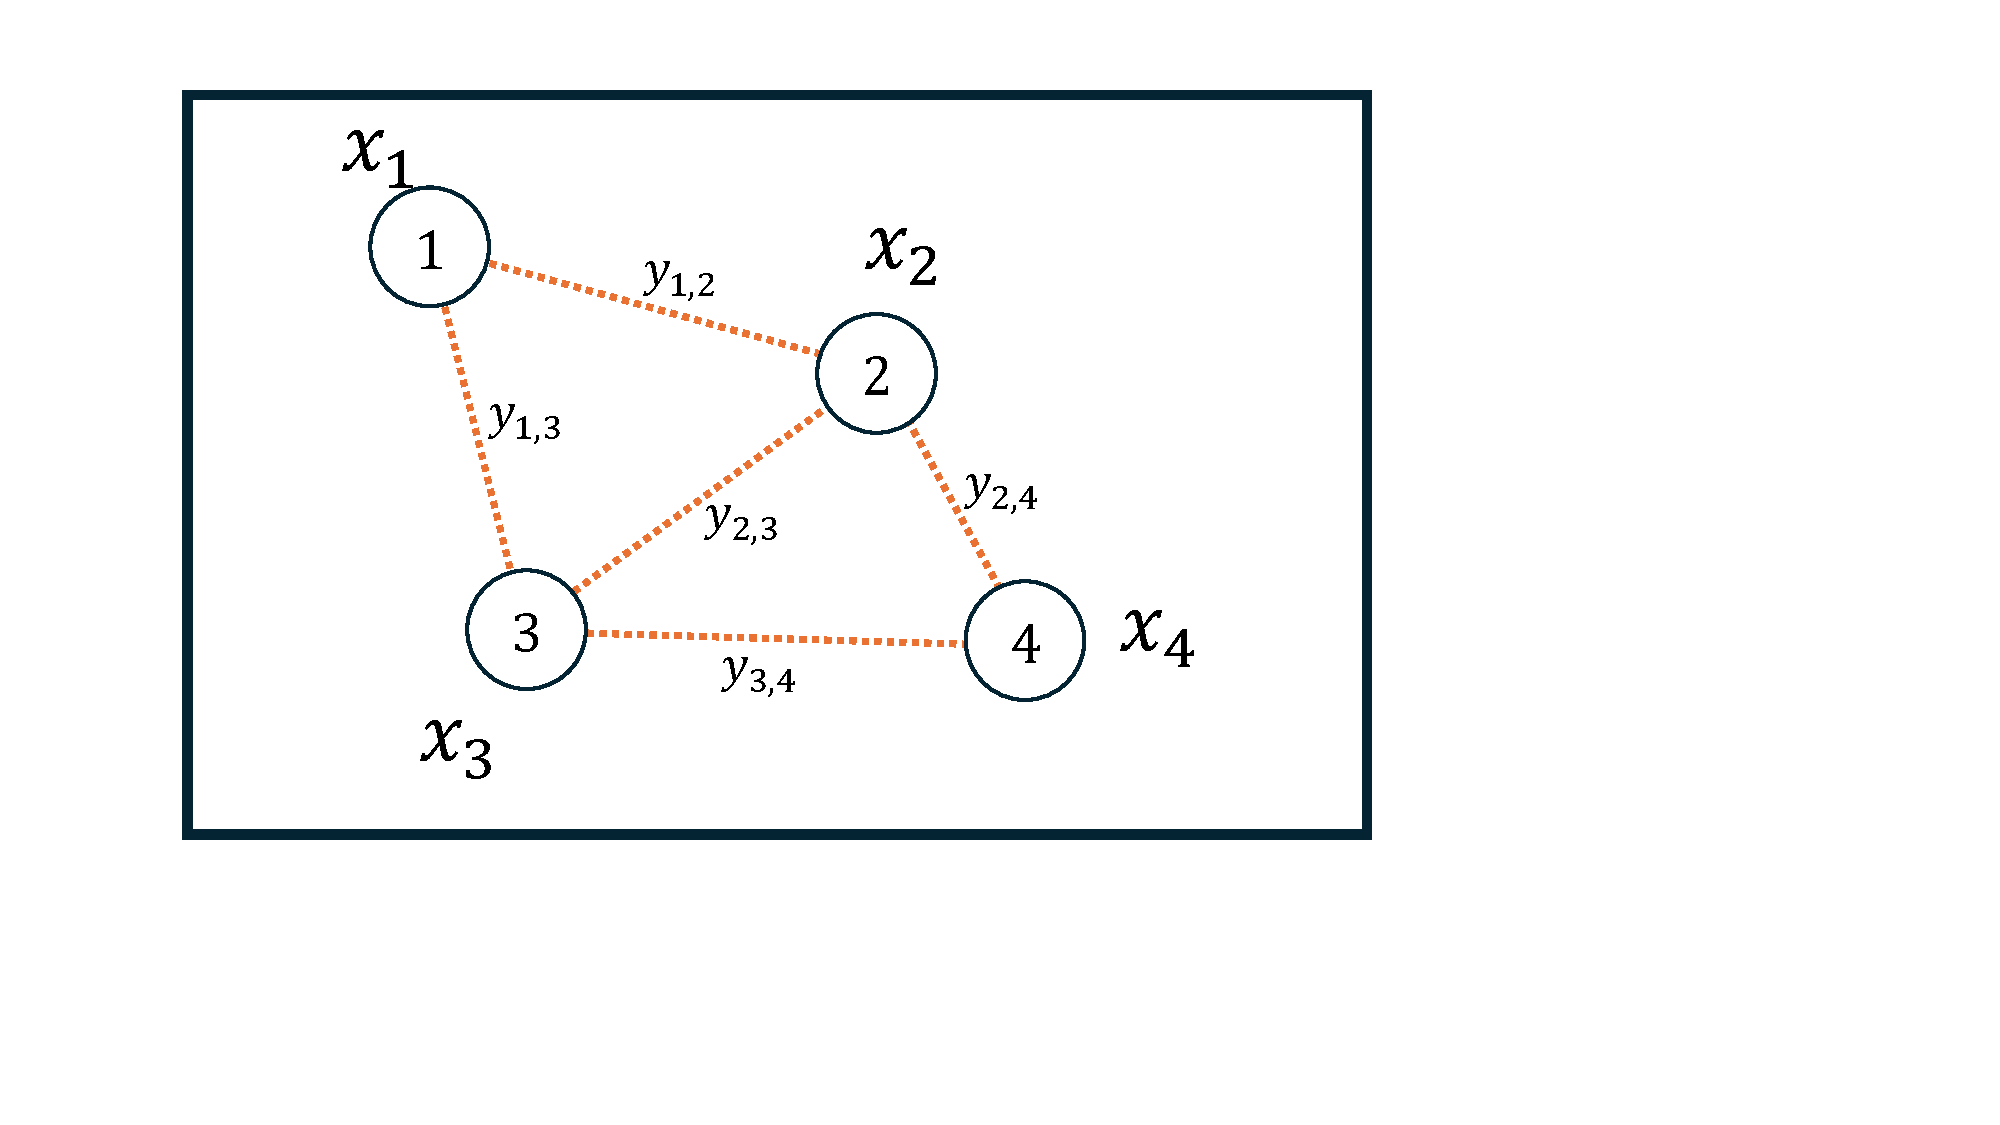
\includegraphics[width=\linewidth,trim=31mm 48mm 106mm 15mm, clip]{graph.pdf}
    \caption{Problem reformulation. In the figure, we have a graph $\mathcal{G}=(\mathcal{V}, \mathcal{E})$ where the directed edges $(i, j) \in \mathcal{E}$ have weights $l_{i,j}$ and the vertices $k \in \mathcal{V}$ have positions $x^{(k)}_t$.}
    \label{fig:problem-graph} 
\end{figure}
As shown in the figure, the graph need not be fully connected, and up to two edges can connect any two vertices, with this representing that two robots have distance measurements of each other. Additionally, the robot distance measurements are assumed to be taken with Gaussian white noise: 
\begin{align}
    y_t^{(i, j)} = l_t^{(i,j)} + U_t^{(i, j)}, \quad U_t^{(i, j)} \sim \text{GWN}(0, \psi_t^{(i, j)})
\end{align}

We use the notation defined in table~\ref{tab:notation} below to describe the graph and the data collected from it.
\FloatBarrier
\begin{table}[ht]
    \centering
    \caption{Additional definitions}
    \label{tab:notation}
    \begin{tabularx}{\linewidth}{lX}
        $\mathbf{J}_t \in \R{m \times 2}$ & 
        \textit{Connectivity matrix}.  Each row $(i, j)\in\mathcal{E}$ represents a directed edge from $i$ to $j$ of the graph. \\
        $\mathbf{y}_t \in \R{m}$ & 
        \textit{Measurement vector}. Each row $k$ is the distance measurement between the two nodes at row $k$ in $\mathbf{J}_t$. \\
        $\bm{\psi}_t \in \R{m}$ &
        \textit{Noise variance vector}. Each row $k$ is the variance of the noise measurement at row $k$ in $\mathbf{y}_t$. 
    \end{tabularx}
\end{table}